\chapter{Methods}
\label{ch:methods}

% Explain what I have done
% - SDR selection
% - testing code (ORCA, emphasize my additions)
% - types of tests performed
% - data visualization tools

% TODO start more gradually
\section{Project Objectives}
\label{sec:project_objectives}
Using a low to mid-range SDR this project aims to detect avalanches and identify targets such as skiers or hikers
to improve avalanche safety.
To do this the avalanche detection system will apply basic Radar principles to identify the location and size of targets.
First, the range data extracted from the frequency differenct from transmit to receive is used to determine distance.
This is mapped to rows projected on the mountainside, where each row represents a distance from the radar.
When samples from the two channels are read into the computer, the computer will apply digital beamforming.
Setting the receivers in the horizontal or azimuth plane is highly effective because it with the range data
the entire mountainside can be mapped.
The beamforming data forms the columns projected onto the mountainside.
The beamforming data combined with the range data forms a grid that is projected on a given mountainside see \ref{fig:mountain_map}.
Then a target can be pinpointed to the physical location on the mountainside.

\begin{figure}[h]
    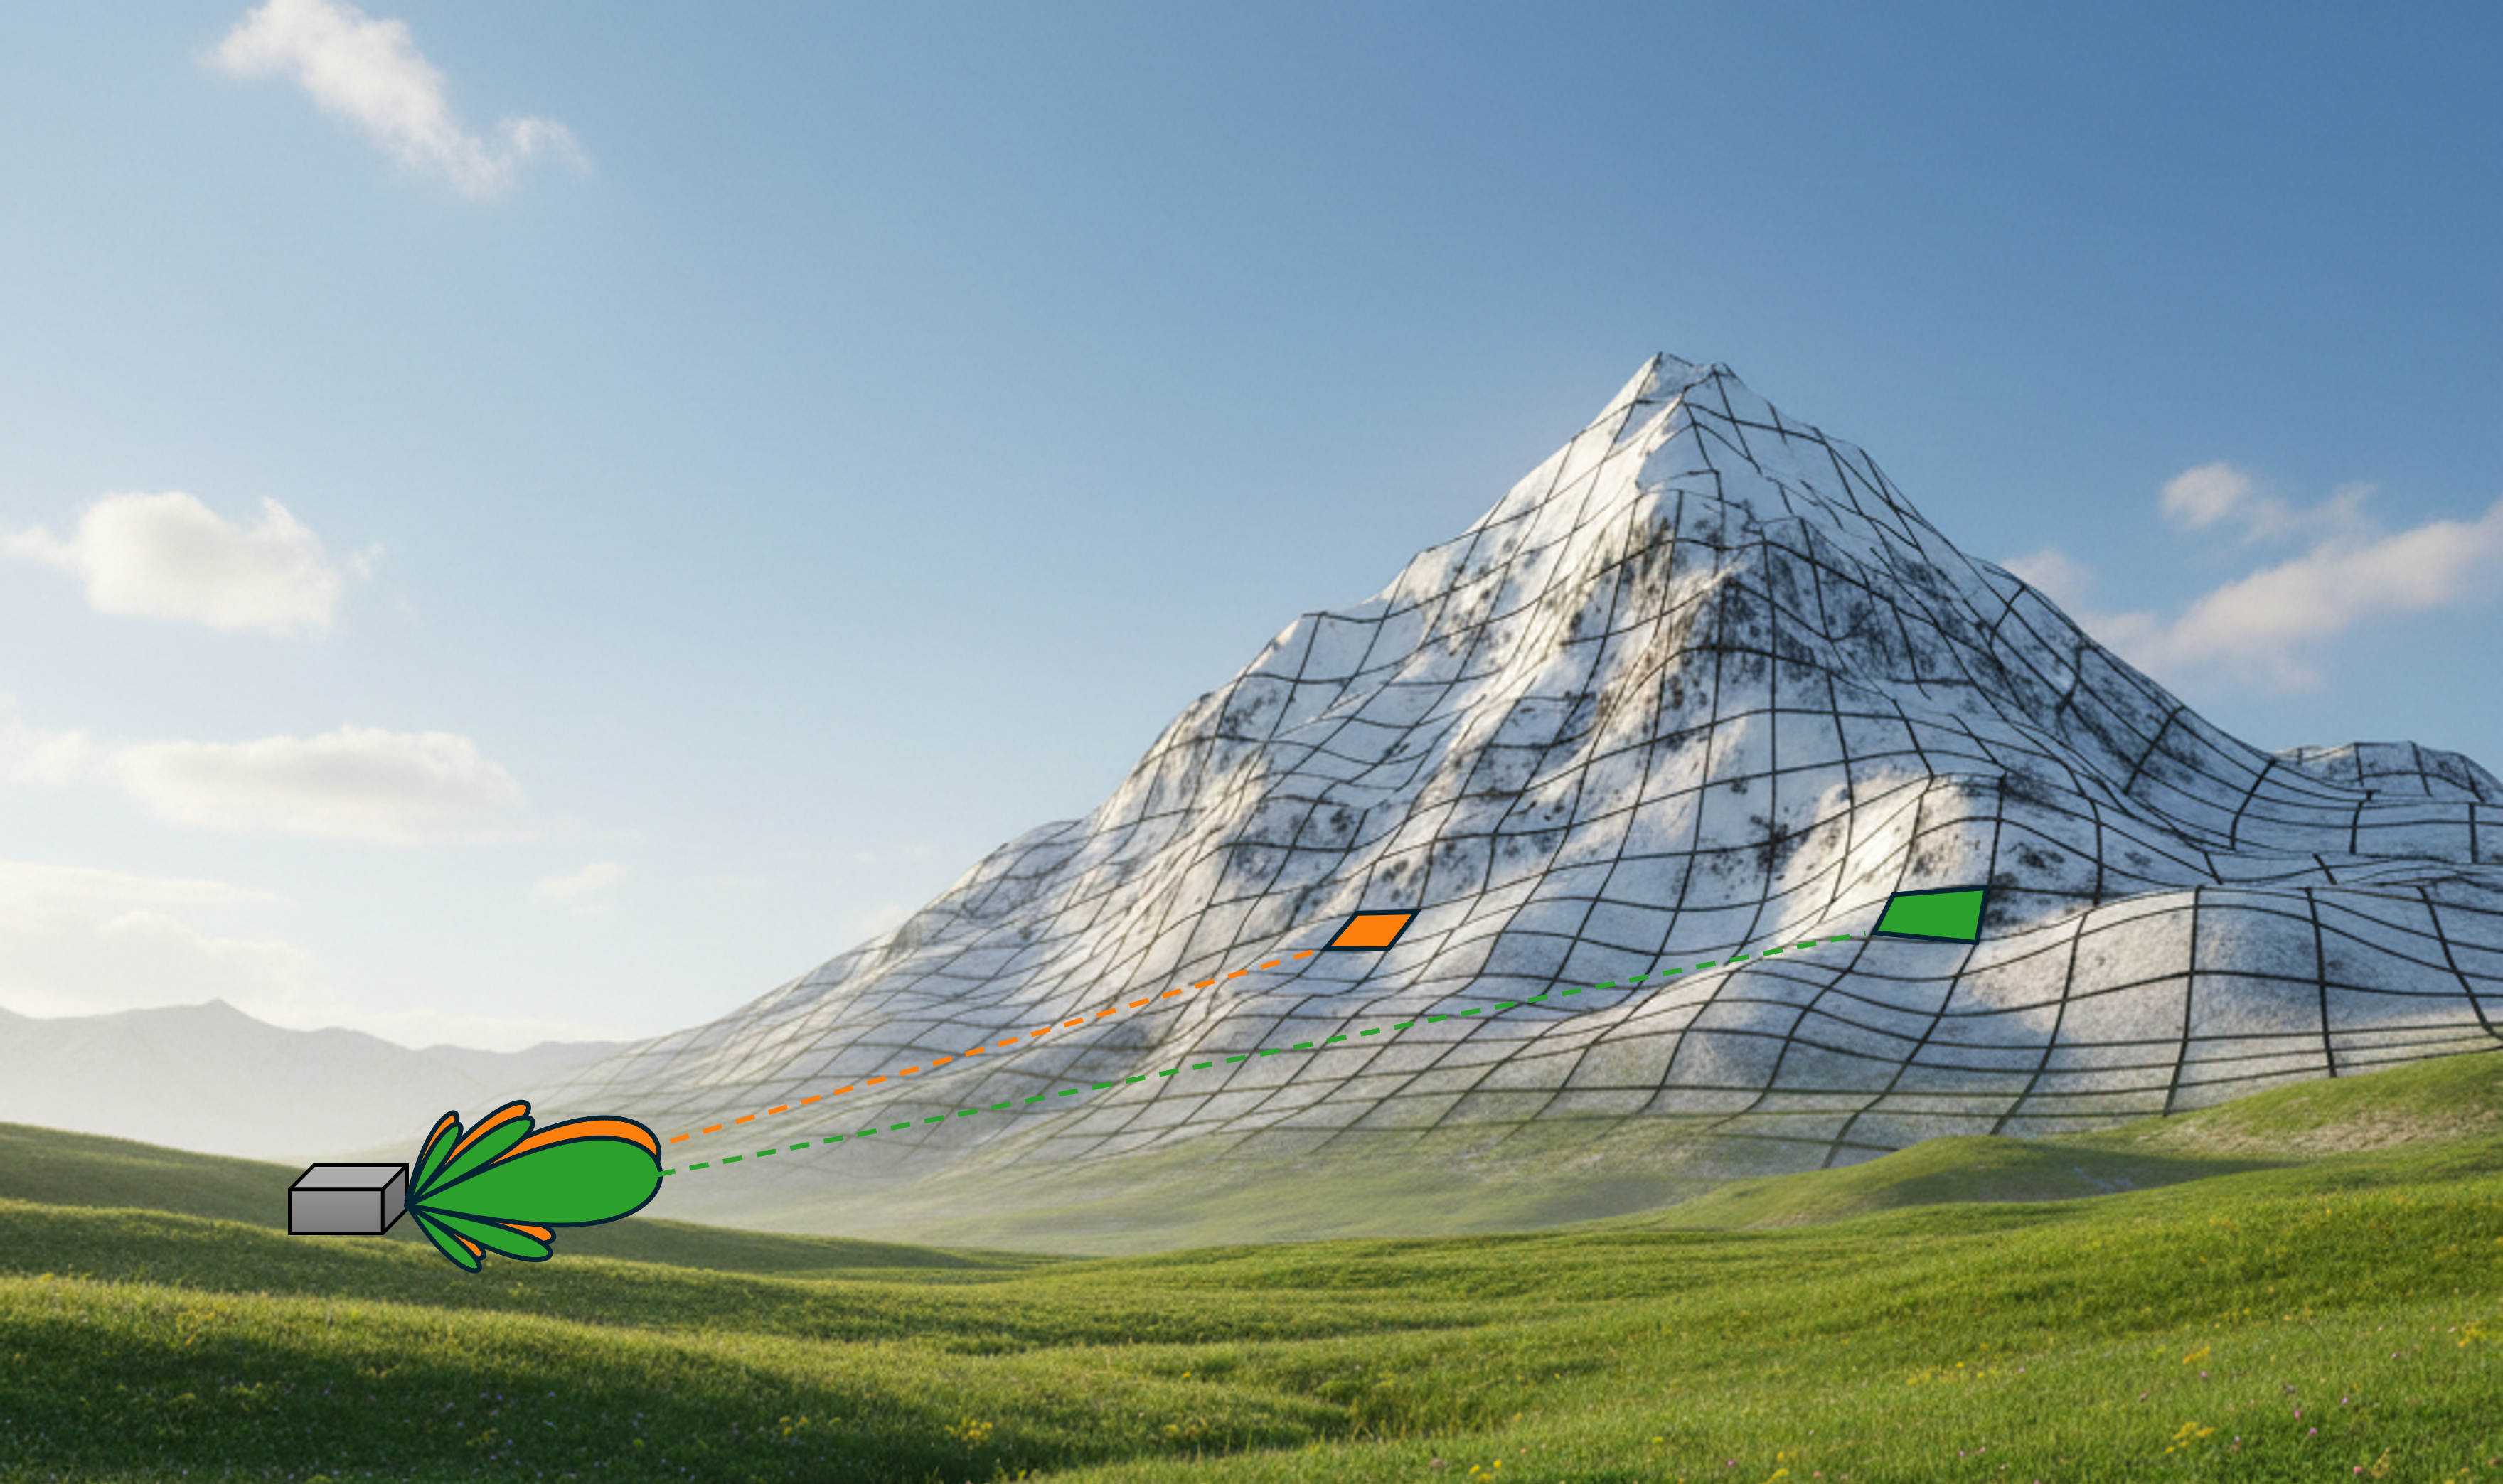
\includegraphics[width=0.9\textwidth, center]{mountainside_map.png}
    \caption{A mountainside (AI generated) with the projected grid from the radar system.
    When a radar target is detected the row is collected from the detected range.
    The column is determined by digital beamforming, with the target appearing at a specific
    angle made from the beamforming.
    The green and oarnge show two different beams and a grid marker on the mountainside
    to the location where a specific angle and range map.}
    \label{fig:mountain_map}
\end{figure}


\section{LimeSDR-Mini}
\label{sec:limesdr}
The avalanche detection project started with a low-end SDR, the LimeSDR-Mini from Lime Microsystems.
This SDR only has one transmit channel and a sample rates of 30.72 MSPS with a frequency range of 10 MHz - 3.5 GHz.
For this SDR we used the software suite SoapySDR which abstracts SDR commands for a
variety of different SDR products and models into one driver interface \cite{noauthor_home_nodate}.
We connected the SDR to two 2.4 GHz horn antennas and a computer to issue commands and collect samples.
Using SoapySDR we collected samples at 2.4 GHz on the LimeSDR-Mini to test its ability as a radar.
Using a corner reflector (which makes a good radar target as all incoming electromagnetic waves are reflected back),
a target was slowly moved away as the SDR collected samples.
Then, using data visualization software generated the FFT of the difference signal for each chirp.
The data shows bright spots where high signal strength was detected.
As the target moved away from the radar the bright showing the corner reflector was detected at further ranges.
A graph of this is shown in \ref{fig:lime_results}.


The LimeSDR-Mini would sometimes miss large amounts of samples which when fed into the data visualizer would create errors and blank spaces in the data.
We found that the LimeSDR had a specific size for the USB data transfer buffers that it used to communicate to the computer.
The data was being sent in sizes that did not match the SDRs buffers, which significantly increased the chance of sample errors.
We redesigned the data transfer to use the hardware buffer size, and it significantly reduced the sampling errors.
Figure \ref{fig:bad_chirps} highlight corrupted samples and the trailing zeroes from the SDR buffers.
This allowed the SDR to be run at a higher sample rates with fewer errors.
We also noticed that the host computer also played a big factor in sample errors,
using a computer such as a Raspberry Pi 4 would significantly increase
sample errors while laptops or desktops would reduce that effect \cite{teisberg_open_2024}.
Figure \ref{fig:old_chirp_send} shows the original data transfer method.
Figure \ref{fig:new_chirp_send} shows the improved data transfer method.
With the improved data transfer method results like figure \ref{fig:lime_results} were collected,
it shows the corner reflector slowly being moved away from the radar.

% TODO improve all captions, they need to describe the image enough to stand on their own
\begin{figure}[h]
    \includegraphics[width=1\textwidth, center]{lime_bad_chirps.png}
    \caption{A collected set of data, in time, showing trailing zeros and corrupted samples.
    Trailing zeros (shown on the right) are a result of the LimeSDR's receive buffer resulting in an
    incomplete dataset that must be filled with zeros to receive the correct amount of samples for proccessing.
    Corrupted samples (shown on the left) occur randomly and ruin a chirp's data.
    Corrupted samples occur more often at higher sample rates, with unoptimized transfer methods and slower computers.}
    \label{fig:bad_chirps}

    \includegraphics[width=1\textwidth, center]{old_chirp_send.png}
    \caption{Original data transfer method using user defined values.
    A chirp is broken down into the individual chunks that are used for USB data transfer.
    USB transmission length is determined by the user, which is unoptimized for the hardware.
    The trailing zeros are included in the transmission.
    This method is very prone to data corruption.}
    \label{fig:old_chirp_send}

    \includegraphics[width=1\textwidth, center]{new_chirp_send.png}
    \caption{Improved data transfer method using hardware optimized values.
    A chirp is broken down into the individual chunks that are used for USB data transfer.
    USB transmission is based on hardware defined values.
    The improved data transfer method also includes an extra data chunk that is discraded 
    to remove the trailing zeros included in the transmission.
    This method significantly reduced data corruption in collected samples.}
    \label{fig:new_chirp_send}
\end{figure}

\begin{figure}
    \includegraphics[width=1\textwidth, center]{lime_results.png}
    \caption{FFT Results of LimeSDR-Mini.
    This data includes null data subtraction to remove the effects of leakage
    (signals directly from the transmitter to the receiver) and stationary targets.
    Zero frequency is near the center of the graph with the x-axis and is proportional to range.
    The chirp number is on the y-axis and is proportional to time.
    The bright patch starting near the center and moving out is the detected corner reflector.}
    \label{fig:lime_results}
\end{figure}


\section{USRP B210}
\label{sec:b210}
The LimeSDR-Mini work was adequate to demonstrate that SDRs could be used in radar applications,
however for Avalanche detection the LimeSDR-Mini's hardware specifications are limiting.
Notably, it only has one channel and a low sample rate.
We decided to switch to a more powerful and expensive SDR:
the Ettus Research USRP B210 as it has two channels and almost double the sample rate.
In addition, the B210's RF properties would make it an improvement over the LimeSDR-Mini.
With the B210 we also decided to switch software tools to the USRP driver as this was the common tool with other projects using this SDR. % TODO awkward

We used a software program called Open Radar Coding Architecture or ORCA \cite{teisberg_open_2024}.
It was a project designed for using SDRs in ground penetrating radar.
It was a valuable tool in collecting data in an organized and configurable way, however, it lacked key features for avalanche detection.
I added changes to allow multichannel data collection and configurations for using the B210 SDR.
For data visualization, ORCA had a few tools that would not work effectively with multiple channels.
I made significant changes and additions to improve data visualization for generating the radar data.

To test the new software tools data was collected using the B210 on its two channels.
Unfortunately when using two channels on the B210 the sample rate must be lowered to 30 MHz
rather than the full 60 MHz that can be used on one channel.
Initial results were collected similarly to the lime SDR where a corner reflector was
slowly moved away from the radar while it collects samples.
The B210 has notable advantages over the LimeSDR being able to operate at a higher frequency (5.8 GHz), collect larger sums of data
and operate on two channels.
